\chapter{Introdución}
\minitoc
\label{chap:introduccion}

%%%%%%%%%%%%%%%%%%%%%%%%%%%%%%%%%%%%%%%%%%%%%%%%%%%%%%%%%%%%%%%%%%%%%%%%%%%%%%%%
% Objetivo: Exponer de qué va este proyecto, sus líneas maestras, objetivos,   %
%           etc.                                                               %
%%%%%%%%%%%%%%%%%%%%%%%%%%%%%%%%%%%%%%%%%%%%%%%%%%%%%%%%%%%%%%%%%%%%%%%%%%%%%%%%

\section{Obxectivo principal}

 \lettrine{O} proxecto que se expón nesta memoria leva por título
 ``\textbf{Deseño e implementación dunha gaita MIDI sen fíos en tempo real
 empregando software/hardware libre}''. \\

 O propio título reflexa bastante ben o que se buscaba con este proxecto.
 Avaliar, analizar, deseñar e implementar de maneira teórico-práctica un 
 controlador MIDI que simule o máis fielmente posible unha gaita galega
 cumprindo cunha serie de requisitos e/ou restriccións:

 \begin{itemize}
  \item Que non empregue fíos.
  \item Que reproduza son en tempo real.
  \item E que empregue exclusivamente hardware e software libre.
 \end{itemize}

 O por qué de todo isto explicarase con calma no capítulo
 \ref{chap:requisitos}.

\section{Outros obxectivos}

 Outros obxectivos secundarios pero non menos importantes que se plantexaron
 durante a realización deste proxecto foron os seguintes:
 
 \begin{itemize}
  \item Realizar un estudio de viabilidade que amosara o que realmente demanda
        o mercado.
  \item Estudar a fondo as tecnoloxías implicadas no proxecto e determinar se
        son aplicables ó mesmo.
  \item Demostrar que o uso de hardware/software libre é viable para este tipo
        de proxectos.
 \end{itemize}

\section{Motivación}

 Son moitos e moi variados os motivos que levaron á realización do presente
 proxecto, a maioría dos cales están presentes no título do mesmo.\\

 O primeiro dos motivos que levou á súa realización foi a idea do mesmo como
 tal, madurada polo proxentando durante máis dunha década, froito da mistura de
 dúas das súas paixóns: a música e a informática. Pero dita idea non sería
 levada a cabo coma Proxecto Fin de Carreira sen o pulo e a motivación por
 parte dos directores do mesmo, que alentaron ó proxectando a levar dita idea
 adiante como tal. \\

 Outro dos motivos que impulsaron o proxecto foi a continua constatación ó
 longo dos anos de que os diferentes productos comerciais que ían saíndo ó
 mercado non cumprían coas expectativas e requisitos que agardaban os
 profesionais da materia. Boa parte desas expectativas e requisitos moitas
 veces solicitados, a maioría dos cales eran obvios, non acabaron de chegar
 nunca, ben por falta de tecnoloxía, ben por falta de coñecementos dos propios
 creadores dos productos. \\

 O continuo fracaso dos mesmo a nivel práctico (que non comercial, onde tiveron
 unha acollida relativamente alta), xunto coa recente aparición de novas 
 tecnoloxías que a priori se poderían aplicar ó producto final, máis os
 coñecementos adquiridos polo proxectando ó longo dos últimos anos, motivaron
 tamén a realización deste proxecto. \\

 Parte deses requisitos e expectativas foron reflexados directamente no título
 deste proxecto: a ausencia de fíos e a xeración de son en tempo real. \\

 Actualmente non existe ningún producto comercial deste tipo que non empregue
 fíos. Probablemente por falta de tecnoloxía no seu momento que garantizase a
 autonomía necesaria e a ausencia de retardos. A principal vantaxe de non
 empregar fíos nunha gaita MIDI é a liberdade de movementos, moi útil por
 exemplo, enriba dun escenario, onde prima o dinamismo. \\

 O seguinte dos motivos xorde da necesidade de cubrir certas áreas do día a día
 no que as gaitas tradicionais frouxean máis ou menos e que as gaitas MIDI
 poden chegar a cubrir aportando certas vantaxes. Entre elas podemos destacar:

 \begin{itemize}
  \item Ensaios no domicilio particular.
        \begin{itemize}
         \item A día de hoxe, ensaiar no domicilio particular en lugares como
               as cidades é pouco menos ca imposible. Se a iso sumamos a
               elevada sonoridade da gaita, podemos dar por seguras as queixas
               veciñais e, de insistir, incluso algunha denuncia por superar os
               decibelios permitidos.
         \item Isto cunha gaita MIDI non pasa, dado que se pode regular o
               volume ou empregar uns cascos para a saída de audio.
        \end{itemize}
  \item Transcripción de melodías.
        \begin{itemize}
         \item Para facer a transcripción dunha melodía para gaita, se só
               contamos cunha gaita tradicional e un ordenador, a transcripción
               hai que facela practicamente a man.
         \item Tendo a man un controlador MIDI pódese conectar ó ordenador e
               xerar a partitura mentres tocamos. Se ese mesmo controlador é
               unha gaita MIDI, aforramos ter que aprender a tocar outro
               instrumento (coma pode ser un teclado) tan só para pasar as
               partituras. Cunha gaita MIDI, a transcripción é totalmente
               natural.
        \end{itemize}
  \item Afinación en condicións desfavorables.
        \begin{itemize}
         \item Para profesionais que adoitan tocar enriba dun escenario en
               calquera época do ano, conseguir afinar correctamente o
               intrumento pode chegar a ser imposible dependendo das condicións
               de temperatura e humidade principalmente.
         \item Neste suposto, a gaita MIDI tamén sae gañando, dado que ditos
               parámetros non lle afectan.
        \end{itemize}
  \item Interpretación en varias tonalidades.
        \begin{itemize}
         \item Hai determinadas pezas nas que o autor recomenda tocar nunha
               tonalidade determinada. Un gaiteiro cun repertorio amplo,
               coñecerá probablemente varias pezas con este tipo de
               restriccións en distinta tonalidade. Se ten que interpretar
               aínda que só sexan un par delas en distinta tonalidade durante
               unha actuación, implicará que ou ben, ten máis dunha gaita
               (maior custe) ou ben precisará andar cambiando de punteiro e de
               bordóns entre peza e polo tanto volver a afinar (ademais do
               tempo que se perde -inasumible-).
         \item Cunha gaita MIDI o cambio de tonalidade é instantáneo.
        \end{itemize}
  \item Interacción automatizada con outros dispositivos MIDI.
        \begin{itemize}
         \item O protocolo MIDI permite enviar mensaxes de sincronización e de
               disparo de eventos, o que á súa vez permite interactuar de
               maneira automatizada con outros dispositivos MIDI que, por
               exemplo, permitirían que un só músico tocando un único
               controlador fixese soar á vez varios instrumentos
               pre-programados e parecer un grupo e non un solista.
        \end{itemize}
 \end{itemize}

 E por último, unha motivación autoimposta: a de facelo empregando
 exclusivamente (sempre na medida do posible e do razoable) hardware e software
 libre. \\

 A día de hoxe tanto o mundo do hardware coma do software libre é un mundo
 maduro que pode competir ó mesmo nivel que o privativo e levar a cabo un
 proxecto coma este, que toca varias ramas da Enxeñería Informática, era unha
 boa ocasión para intentar demostralo. \\

 Ademais, fomentar o coñecemento e a cultura libre debería ser o habitual no
 ámbito da educación, no que se engloba o ensino universitario. Compartir o
 coñecemento fomenta a colaboración e o pensamento crítico e, no tocante a este
 proxecto, pode xerar unha comunidade arredor do mesmo. \\

 E xerar unha comunidade de colaboradores debería redundar na mellora do
 proxecto a longo prazo, do que se poderían beneficiar todos os interesados. \\

 Se o levamos ó terreo económico, redunda na mellora dun producto comercial,
 que pode incrementar as vendas e ó mesmo tempo mellorar a satisfación dos
 clientes. \\

 Se o levamos ó terreo cultural, contribúe á conservación da cultura e tradición
 galegas. E iso é beneficio para todos. \\

 Seguindo estes principios, o contido deste proxecto atópase dispoñible baixo a
 licencia GPLv3 (e CC-BY-SA para contidos non licenciables baixo GPLv3) no
 enderezo \url{http://proxecto-puding.org/}. Así mesmo, co fin de xerar
 %enderezo http://proxecto-puding.org. Así mesmo, co fin de xerar
 comunidade arredor do proxecto, existen unha serie de contas de promoción en
 redes sociais e unha rolda de correo accesibles desde o mesmo enderezo.

\section{Visión xeral do sistema}

 Aínda que máis adiante se explicará en detalle, convén dar unha visión xeral
 do sistema para comprender os seguintes capítulos. \\

 Esquematicamente falando, o deseño conceptual do sistema ó que se pretendía
 chegar era o seguinte (figura \ref{figura:DesenoConceptual}).

 \begin{figure}[htbp]
  \centering
  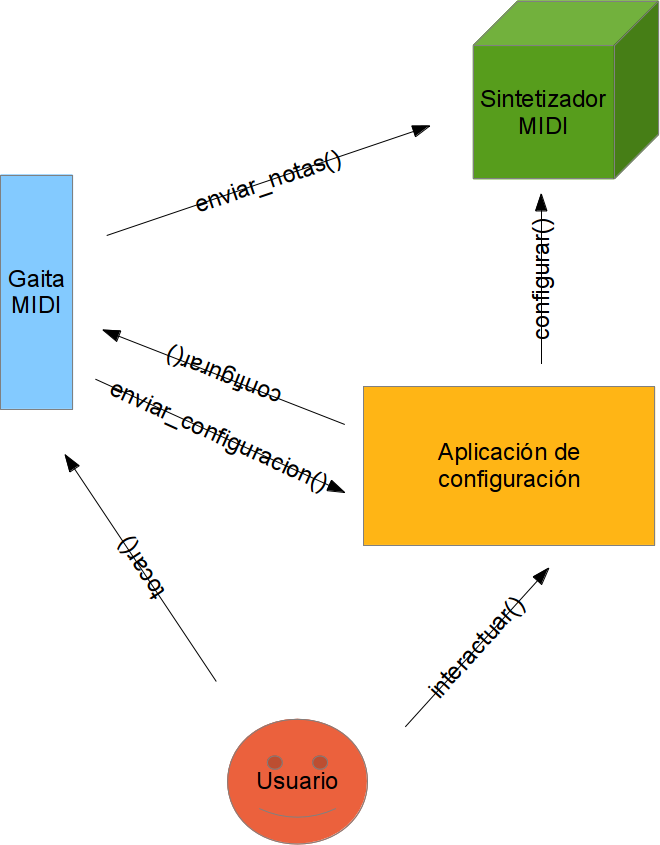
\includegraphics[scale=0.6,keepaspectratio=true]{./imagenes/concepto-operacion.png}
  % concepto-operacion.png: 660x845 pixel, 96dpi, 17.46x22.35 cm, bb=0 0 495 634
  \caption{Deseño conceptual do sistema}
  \label{figura:DesenoConceptual}
 \end{figure}

 Na figura obsérvase un sistema composto por catro elementos ou actores, sendo
 un deles o propio usuario. \\

 Dos tres restantes, o situado á esquerda correspóndese coa parte hardware e os
 situados á dereita, coa parte software. \\

 O usuario será o encargado de tocar a gaita (ou controlador) MIDI, que enviará
 a melodía ou conxunto de notas ó sintetizador MIDI, que se encargará de
 reproducilas. \\

 Así mesmo, poderá modificar a configuración de calquera dos dous elementos
 (dependendo dos parámetros modificados) a través dunha interface gráfica, a
 aplicación de configuración. \\

 Cando a aplicación de configuración detecte algún controlador MIDI conectado
 encargarase de rexistralo e amosar a configuración persoal que este lle envíe,
 información que será vista polo usuario e que logo poderá modificar a vontade.
 
\section{Métodos e fases do proxecto}

 Tendo claro hacia onde ía encamiñado o proxecto, procedeuse a acometer o mesmo
 en diferentes fases. \\

 Nunha primeira fase analizouse a viabilidade do proxecto, incluíndo un estudo
 da viabilidade do mesmo, que abranguiu desde o estudo das solucións xa
 existentes ata a realización dunha enquisa entre os posibles usuarios, pasando
 por un primeiro prototipo. \\

 Nunha segunda fase analizarónse os requisitos, facendo uso dun estudo das
 solucións xa existentes, dun segundo prototipo aparentemente funcional e da
 enquisa previa para a extracción de requisitos por parte do proxectando, por
 parte de expertos e por parte de usuarios anónimos a través de simulacións,
 modelos e programas de proba. \\

 Nunha terceira fase acometeuse o deseño. Previo estudo das tecnoloxías a
 empregar a priori (Arduino, MIDI, etc.), fíxose un terceiro prototipo
 (hardware e software) a partir do que se obtivo un primeiro deseño.\\

 Nunha cuarta e última fase acometeuse o desenvolvemento. Unha vez obtido o
 deseño inicial, obtívose un prototipo operacional sobre o que realizar máis
 probas e que deu lugar a un deseño máis detallado, que se empregou para a
 construcción e implementación do producto final, que foi probado e refinado
 mediante as pertinentes probas de unidade e integración. \\

 En todas as fases houbo tamén un apartado de determinación de obxectivos,
 avaliación de alternativas e resolución de riscos, coa fin de asentar as bases
 de cada unha e de prever posibles problemas. \\

 Finalizado todo este proceso obtívose o producto final, así coma unha serie de
 conclusións que levarán a obter diferentes melloras futuras do mesmo.

\section{Estructura da memoria}

 A división e transcurso do proxecto seguiu as liñas mestras que se expoñen na
 presente memoria, articulada en dous grandes bloques:

 \begin{enumerate}
  \item \textit{Contextualización e traballos previos}. Neste apartado
        inclúese unha breve pincelada histórica da gaita galega, a súa
        composición, os principais protocolos que se empregaron no proxecto e
        o estado da arte actual.
        
  \item \textit{Desenvolvemento do caso de estudo}.
        \begin{enumerate}
         \item Análise da viabilidade.
         \item Análise dos requisitos.
         \item Deseño do sistema.
         \item Desenvolvemento do sistema.
        \end{enumerate}
 \end{enumerate}

 Inclúense tamén varios anexos con información complementaria relativa ó
 proxecto que, por extensión, son dificilmente intercalables nos apartados
 previos.
